    The results of steady-state optimizations give very valuable information about the desired operation of
    the process in question. In real-live applications however, processes will always display transient behaviour,
    which cannot be captured by steady-state models. Any given process is required
    to operate within ceratin bounds and subject to external disturbances, which might cause the process to deviate
    from desired operations. To be able to handle such disturbances, or in some cases even be able
    to operate at all at the specified operating point, control structures are required. By the nature of the question 
    aspects of stability or operability can only be analyzed based on a dynamic representation of the system. 

    The consideration of dynamics further opens the possibility to extend the optimization beyond monetary measures, or
    consider transient aspects which play a role in process profitability. This might include the optimization of transition
    times between multiple steady states, or an improved start-up or shut down behaviour. The product streams from a process 
    during transition times often have to be discharged. By optimizing the transition process, one might be able produce 
    marketable or usable product, even during transitions. In case of the ASU which might also be implemented as a utility 
    to a downstream process, the load following behaviour according to utility requirements could also be analyzed.
    
    The remainder of this section is structured as follows. Initially, the dynamic degrees of freedom for the ASU
    flowsheet are discussed. Subsequently the dynamic process behaviour is analyzed with regards to the sensitivity 
    to external and internal disturbances. Some conclusions are drawn from the observed dynamic effects, encountered 
    particularly in high purity distillation processes. 

    \subsection{Degrees of freedom}
        In order to gain more insight into the behaviour of the dynamic models presented above an analysis
        of the degrees of freedom within the model is at hand. For the degrees of freedom the cost correlations
        will be disregarded, as they for a closed system of equations given the inputs generated form the column
        model. Furthermore interdependencies can be disregarded, as the cost model consist only of ''forward''
        computations. In practical terms this statement can be confirmed since the models can be evaluated
        with and without costing equations. Hence only the stage and hydraulic equations will be considered.

        For a given column without condenser or reboiler the model is made up of $[n_S (5n_C + 24) + n_F]$
        differential algebraic equations in $[n_S (5n_C + 29) + n_F (n_S + n_C + 3) + 1]$ variables. In this
        isolated case all feed flow rates, their composition and enthalpies would be specified. In this case
        the feeds include a hypothetical condenser reflux (the upper most feed) as well as reboiler reflux
        (lowest feed). Along with the feeds and their qualities, the feed splits and reflux split have to be
        assigned. Lastly the column diameter needs to be known. This yields $[n_F (n_S + n_C + 2) + n_S + 1]$
        specifications. To close the system initial conditions for all states have to be given. There
        are a total of $[4 n_S ]$ dynamic states in a column section.

        The condenser reboiler unit is made up of a total condenser and a reboiler side. For the condenser side
        holdups are neglected. While the reboiler side is modeled much like a column stage. The complete model
        consists of $[14 + 6 n_C]$ equations in $[17 + 6 n_C]$ variables. The three specified variables would
        commonly correspond to the condenser pressure, reboiler volume and reflux ratio on the condenser side.
        While other specifications are conceivable, they cannot be made entirely arbitrarily. A specification
        on the reboiler pressure for instance would result in a high index problem ($\approx n_S^{LPC}$) which
        could not be solved without drastically reformulating the model.

    \subsection{Dynamic process behaviour}
        With the dynamic models a more rigorous approach to analysing the process behaviour is possible.
        Several aspects of the transient behaviour are of interest. To gain an insight into the process dynamics
        and test the capabilities of the implemented models, several simulation studies have been conducted.

        Especially when dealing with control aspects of a process, the step responses to disturbances in the
        process are of great interest. Therefore first a study of process reactions to various internal and
        external disturbances will be conducted. This is followed by a more detailed investigation of some phenomena
        occurring during process operations.


        \subsubsection{Step responses}
            To identify a possible control structure the dynamic interactions of the process have to be analyzed.
            The most current method of controlling a process would be model predictive control (MPC), where
            the set point for all manipulated variables are provided by a central controller, which is based
            on a rigorous process model. In this case however a simpler and in practice still more common
            approach is to implement PID control loops. In that case each measured variable is paired
            with a manipulated variable, which is altered to keep the measured quantity within operational
            bounds.

            Among the most tested tools to synthesize a control structure are the relative gain array (RGA) and block
            relative gain (BRG). Those tools provide a measure for the interactions within the process. As it
            is unlikely, that one manipulated variable will only affect the controlled variable it is assigned to.
            Intuitively, highly integrated processes display strong interactions between all manipulated and
            measured variables. To analytically calculate the RGA or BRG, a control (linearized) process model
            in terms of transfer functions is necessary. Alternatively, plant or simulation experiments can be used, 
            to determine the interdependencies within the process. To do so, the process response in the controlled 
            variables to step changes in manipulated variables is examined. 

            To derive feasible pairings, first all manipulated ($u_i$) and measured ($y_i$) variables are identified, 
            based on the previously discussed degrees of freedom. The measured variables correspond to the constraints 
            enforced on the process.
            \begin{itemize}
                \item $y_1$ : LPC nitrogen purity $\left(y_{1,N_2}^{LPC}\right)$
                \item $y_2$ : oxygen product purity $\left(x_{O_2}^{CR main}\right)$
                \item $y_3$ : CAC argon purity $\left(y_{1,Ar}^{CAC}\right)$
                \item $y_4$ : nitrogen product flowrate $\left(\dot{n}_{N_2}\right)$
                \item $y_5$ : oxygen product flowrate $\left(\dot{n}_{O_2}\right)$
                \item $y_6$ : argon product flowrate $\left(\dot{n}_{Ar}\right)$
            \end{itemize}

            The manipulated variables are derived from the degrees of freedom analysis.
            \begin{itemize}
                \item $u_1$ : main air feed flowrate $\left(\dot{n}_{air}\right)$
                \item $u_2$ : CR main reflux ratio $\left(\nu^{CR main}\right)$
                \item $u_3$ : CR CAC reflux ratio $\left(\nu^{CR CAC}\right)$
                \item $u_4$ : HPC side stream flowrate $\left(S^V_1\right)$
                \item $u_5$ : LPC side stream flowrate 1 $\left(S^V_1\right)$
                \item $u_6$ : LPC side stream flowrate 2 $\left(S^V_2\right)$
            \end{itemize}

            To analyze the impact of the different manipulated variables, several simulation studies were
            undertaken. The steady state attained during steady state optimization was taken as nominal operating
            conditions. To get a feel for the process behaviour, the responses to a $10 \%$ step increase in
            the manipulated variables was simulated. The results are displayed in \figref{fig:opt:stepresp}.

            Before discussing the results in more detail, some comments have to be made as to how these results
            were attained, and how they are displayed. While for most cases the step response simulation was
            straightforward, it did lead to errors for the vapour side draw from the high pressure column. To still
            produce usable data, a steep ramp was used alternatively. Over a time-interval of 10 seconds, the nominal
            value was increased  by ten percent, and remained steady afterwards. To produce a meaningful and comparable
            representation of the simulation results, all values for the measured variables were normalized to their
            respective values under normal operating conditions. Furthermore there are two time scales employed, indicated
            on the bar below the graphs. All cases were simulated for the span of an entire day, and the step was applied
            at the very beginning of the simulation. When analysing the results, it turned out, that dynamic effects were
            taking place on two different scales. While some measured variables were only approaching steady-state
            at the end of the day, others reached it within about an hour. The different time scales are due to the
            nature of the measured variables. Pressure associated values such as flowrates change much more quickly,
            than temperature or concentrations \cite{Roffel.2000}. It also needs to be pointed out, that the y-scales
            for the graphs differ between measured variables. To maintain some degree or comparability,
            the y-scales are constant for each measured variable. In the given process configuration, the changes
            inflicted by the applied steps are of rather low amplitude. For the considered concentrations, the changes
            to the order of $10^-{3}$ or 0.1 \% were observed. Non the less, given these responses, preliminary candidates
            for coupling between controlled and measured variables can be deduced.

            \begin{landscape}
                \begin{figure}
                    \center
                    % GNUPLOT: LaTeX picture with Postscript
\begingroup
  \makeatletter
  \providecommand\rotatebox[2]{#2}%
  \@ifundefined{ifGPcolor}{%
    \newif\ifGPcolor
    \GPcolortrue
  }{}%
  \@ifundefined{ifGPblacktext}{%
    \newif\ifGPblacktext
    \GPblacktexttrue
  }{}%
  % define a \g@addto@macro without @ in the name:
  \let\gplgaddtomacro\g@addto@macro
  % define empty templates for all commands taking text:
  \gdef\gplbacktext{}%
  \gdef\gplfronttext{}%
  \makeatother
  
  \setlength{\unitlength}{1cm}%
  \begin{picture}(23.8,16)%
    \gplgaddtomacro\gplbacktext{%
        \put(0,1.75){\makebox(0,0)[r]{\strut{} $u_6$}}%
        \put(0,4.25){\makebox(0,0)[r]{\strut{} $u_5$}}%
        \put(0,6.75){\makebox(0,0)[r]{\strut{} $u_4$}}%
        \put(0,9.25){\makebox(0,0)[r]{\strut{} $u_3$}}%
        \put(0,11.75){\makebox(0,0)[r]{\strut{} $u_2$}}%
        \put(0,14.25){\makebox(0,0)[r]{\strut{} $u_1$}}%
        \put(2.4,16){\makebox(0,0)[cr]{\strut{} $y_1$}}%
        \put(6.2,16){\makebox(0,0)[cr]{\strut{} $y_2$}}%
        \put(10,16){\makebox(0,0)[cr]{\strut{} $y_3$}}%
        \put(13.8,16){\makebox(0,0)[cr]{\strut{} $y_4$}}%
        \put(17.6,16){\makebox(0,0)[cr]{\strut{} $y_5$}}%
        \put(21.4,16){\makebox(0,0)[cr]{\strut{} $y_6$}}%
        \put(0.5,0.25){\line(1,0){22.8}}
        \put(0.5,0.15){\line(0,1){0.2}}
        \put(4.3,0.15){\line(0,1){0.2}}
        \put(8.1,0.15){\line(0,1){0.2}}
        \put(11.9,0.15){\line(0,1){0.2}}
        \put(15.7,0.15){\line(0,1){0.2}}
        \put(19.5,0.15){\line(0,1){0.2}}
        \put(23.3,0.15){\line(0,1){0.2}}
        \put(2.4,0){\makebox(0,0)[c]{\strut{}  \footnotesize $1 d$}}%
        \put(6.2,0){\makebox(0,0)[c]{\strut{} \footnotesize $1 d$}}%
        \put(10,0){\makebox(0,0)[c]{\strut{} \footnotesize $1 d$}}%
        \put(13.8,0){\makebox(0,0)[c]{\strut{} \footnotesize $5000 s$}}%
        \put(17.6,0){\makebox(0,0)[c]{\strut{} \footnotesize $5000 s$}}%
        \put(21.4,0){\makebox(0,0)[c]{\strut{} \footnotesize $5000 s$}}%
    }%
    \gplgaddtomacro\gplfronttext{%
    }%
    \gplbacktext
    \put(0.5,0.5){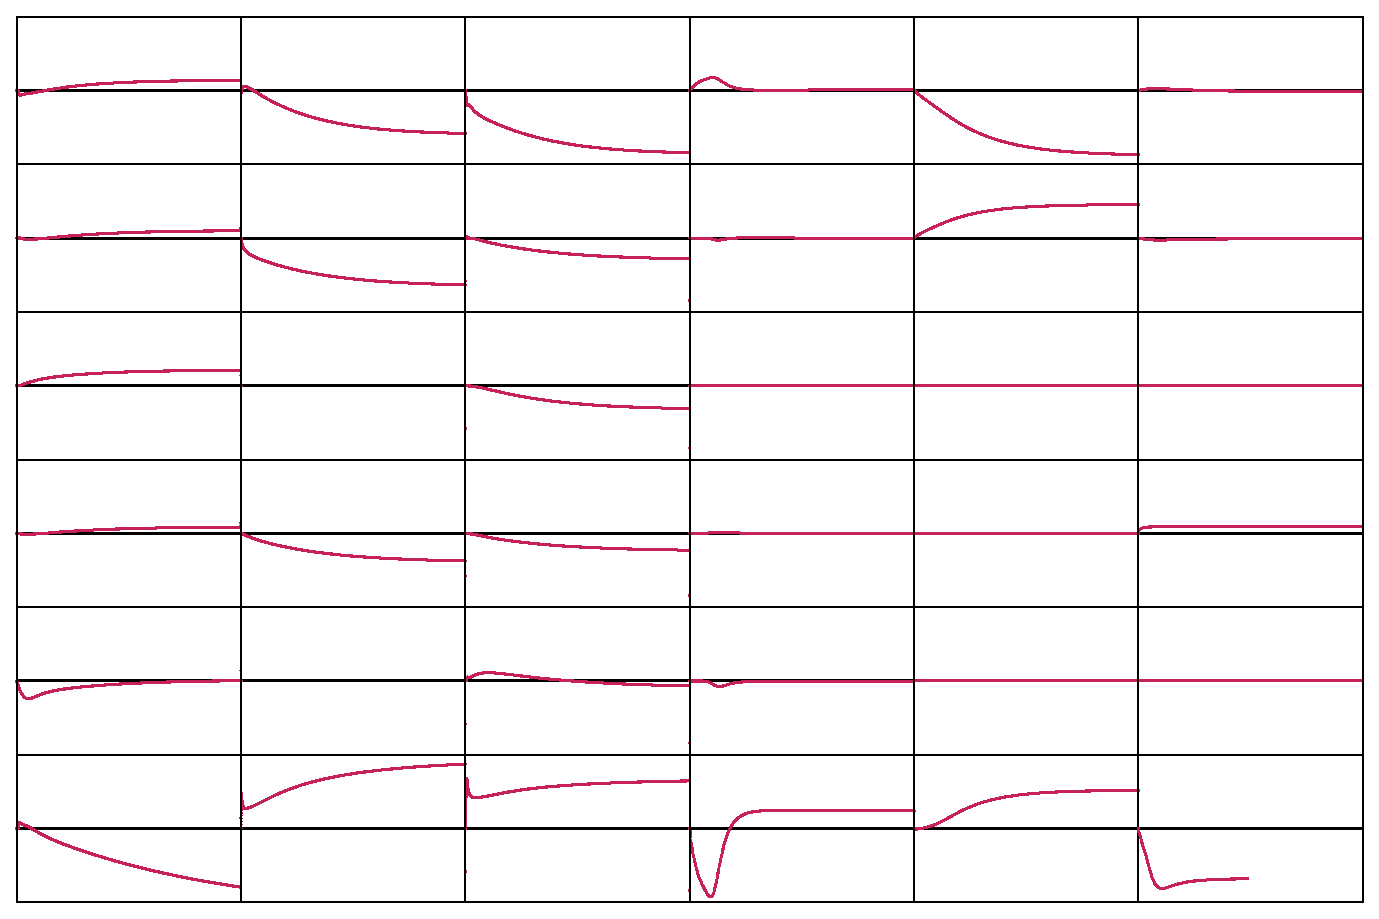
\includegraphics{GNUPlot/B1_Plot}}%
    \gplfronttext
  \end{picture}%
\endgroup

                    \caption{step responses.}
                    \label{fig:opt:stepresp}
                \end{figure}
            \end{landscape}

        \subsubsection{Dynamic profiles}
            The previous section showed only minor reactions to step changes in the manipulated variables. However
            a closer look at the dynamic column profiles reveals a much different picture. To analyze the internal
            column behaviour a external disturbance to the feed pressure was applied. As a result, the concentration
            profiles within the column undergo various changes. Especially with high purity separation sequences,
            a highly non-linear behaviour with two distinct characteristics is displayed. For one, two time scales can
            be observed, in which new steady states are reached. Secondly, the transition time
            between two steady states relies heavily on direction and magnitude of the disturbance \cite{Hwang.1991}.
            The first effect deals with short- and long-term dynamics, while the second is referred to as asymmetric dynamics.

            \begin{figure}
                \scriptsize
                \center
                \begin{subfigure}{0.48\textwidth}
                    \input{GNUPlot/N2_ADyn_plus}
                    \caption{Dynamic profile after feed enthalpy increase.}
                    \label{fig:N2_ADyn_plus}
                \end{subfigure}
                    \begin{subfigure}{0.48\textwidth}
                    \input{GNUPlot/N2_ADyn_minus}
                    \caption{Dynamic profile after feed enthalpy decrease.}
                    \label{fig:N2_ADyn_minus}
                \end{subfigure}
            \end{figure}

            From this preliminary study, of the dynamic process behaviour, it can be concluded, that an effective control strategy,
            should not only aim at directly maintaining the the product qualities, but rather to stabilize the internal column
            profiles. As the effects are often on time scales spanning over a day, there is a chance to detect malicious effects to
            product specifications in advance and and introduce appropriate counter measures. As can be seen in \figref{fig:N2_ADyn_plus}
            the external disturbance leads to formation of a concentration wavefront within the column. This behaviour is typical 
            for septation processes and be exploited to derive low-order models for control purposes \cite{Marquardt.1988}. 
            The fact that this non-linear behaviour is captured by the implemented models, further deepens the trust in the predictive
            capabilities of the implemented models. 






